\chapter{Modeling}
Steve is a good model~\citep{stevewiki}.
He has a fancy suit, see Figure~\ref{figure:fancysuit}.
He wrote a good paper~\citep{robinson1991coherent}.

\begin{figure}[tb]
    \begin{center}
        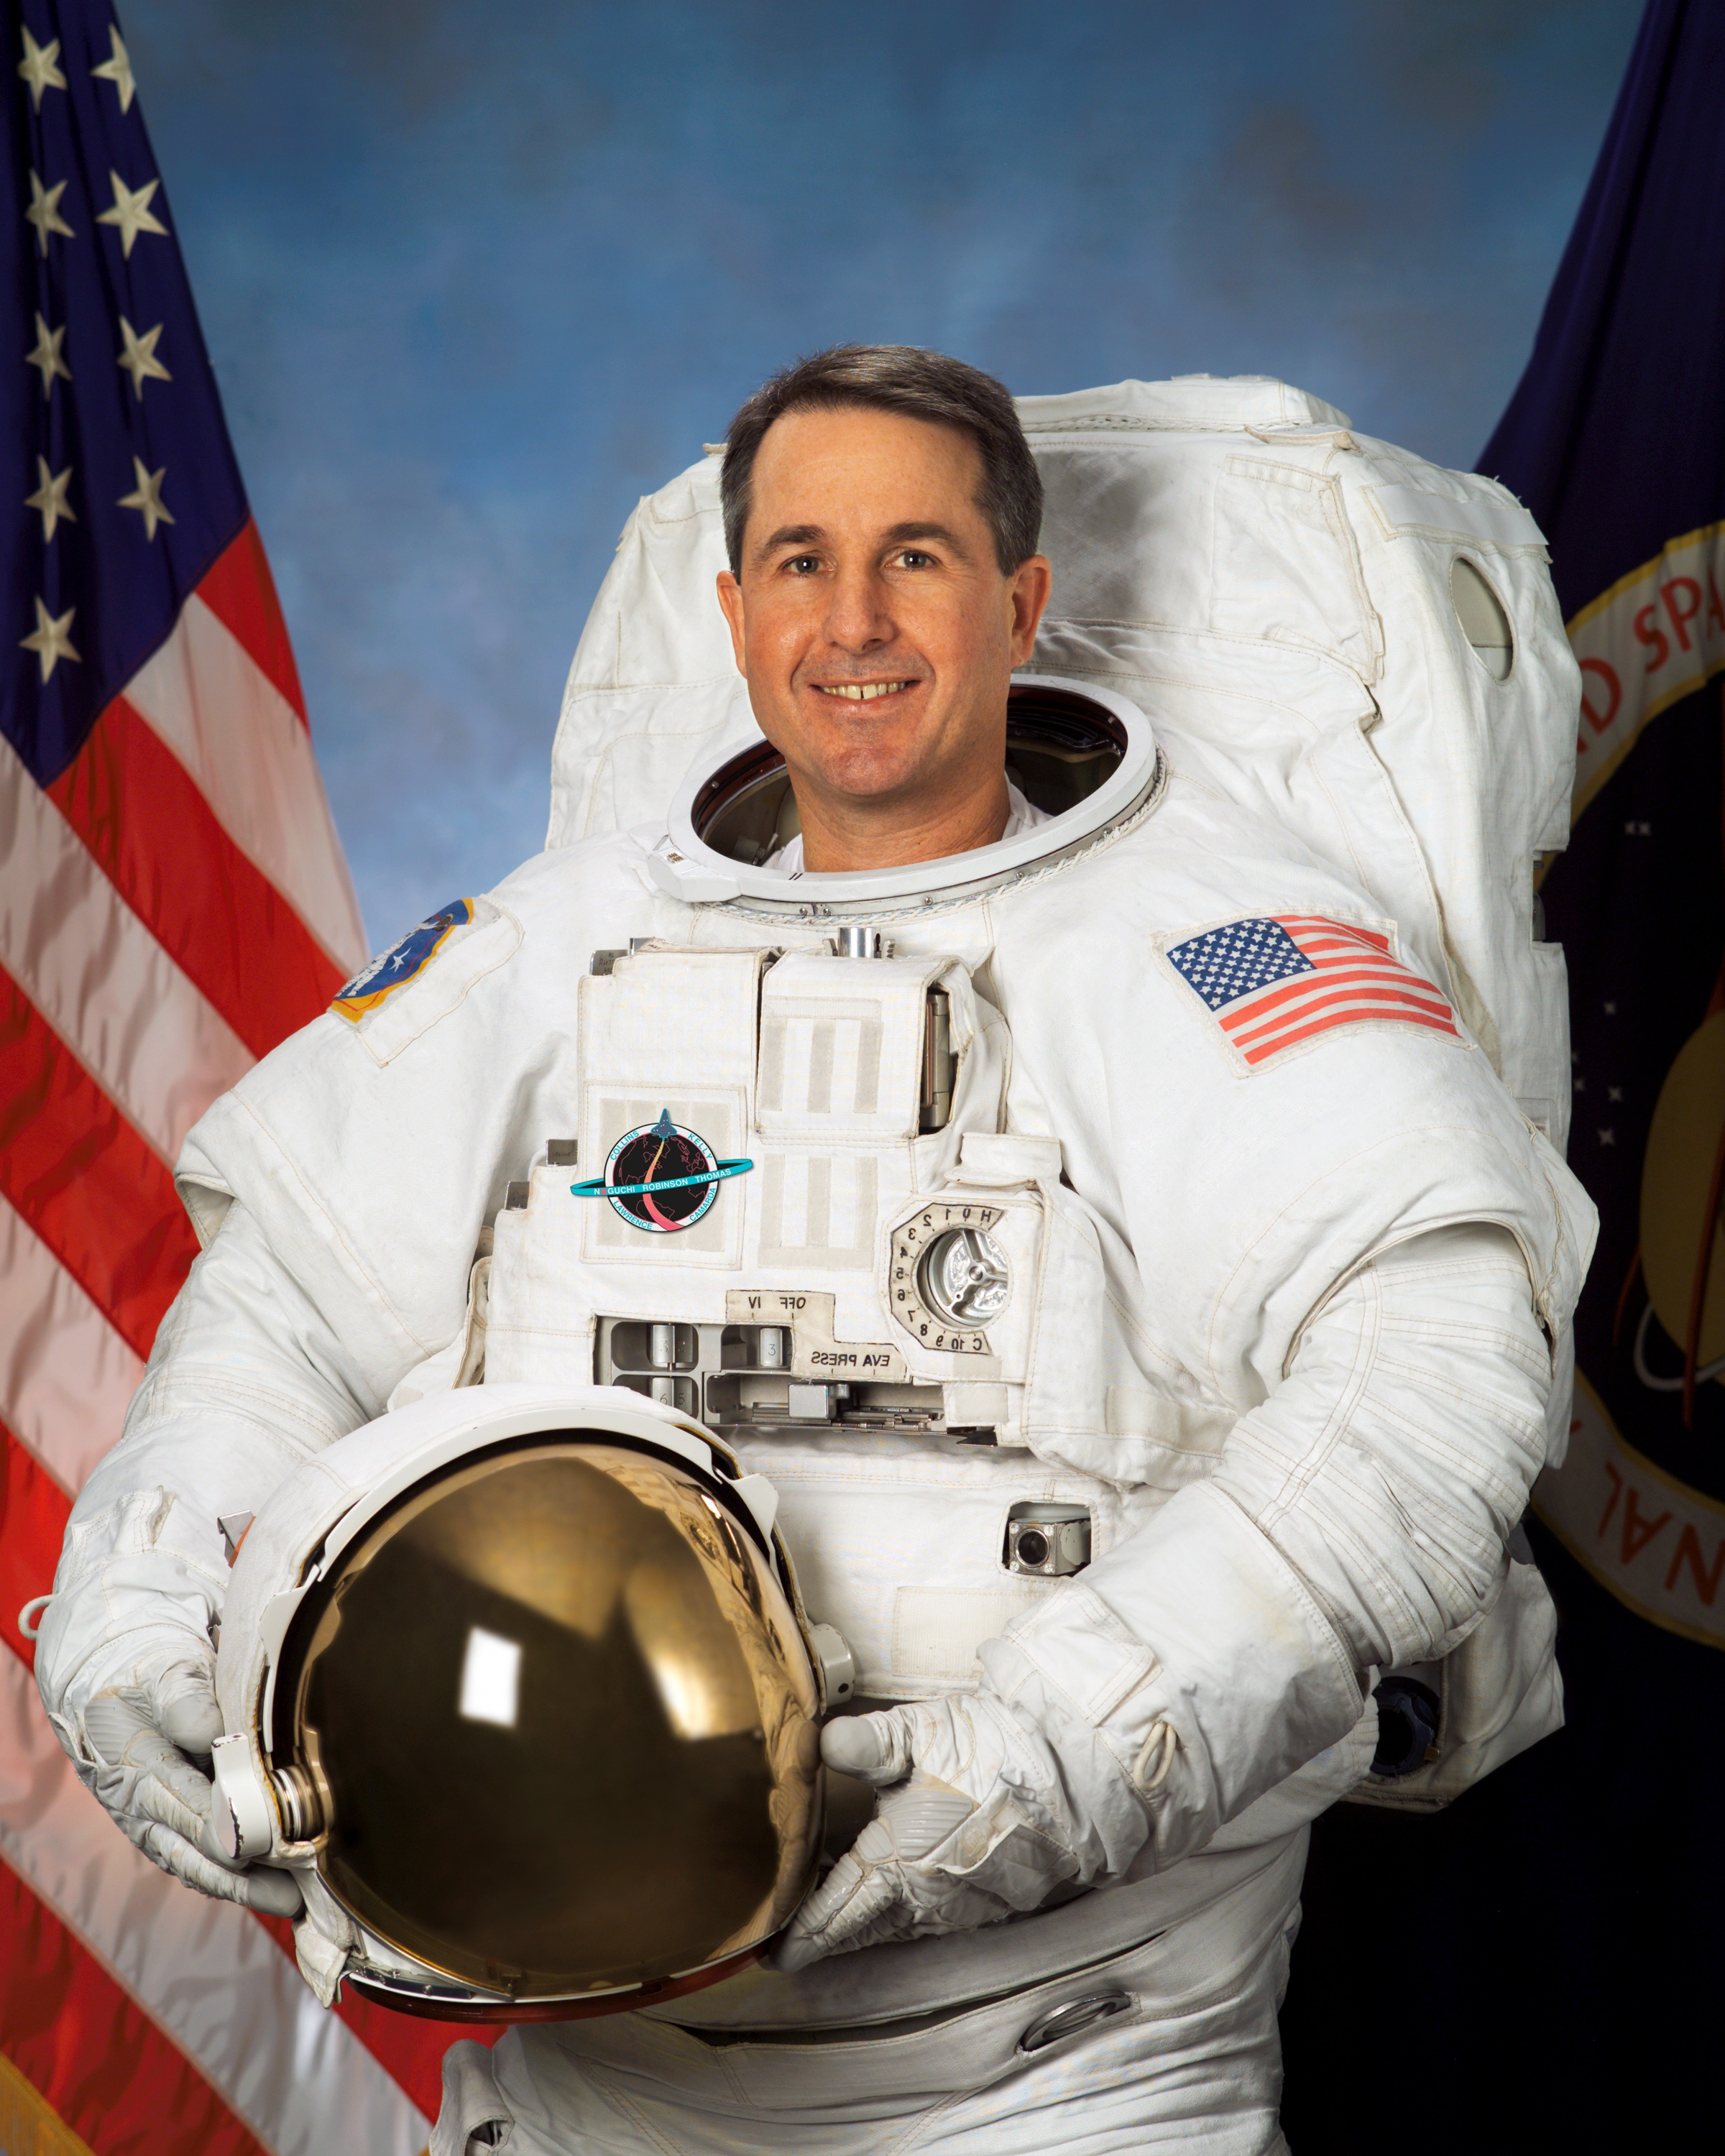
\includegraphics[width=0.25\linewidth]{figures/Modeling/Stephen_Robinson_NASA_STS114.jpg}
        \caption[Fancy suit man]{Astronaut Stephen K. Robinson, mission specialist}
        \label{figure:fancysuit}
    \end{center}
\end{figure}

\section{Introduction}
Stephen Kern Robinson (born October 26, 1955, in Sacramento, California) is a former NASA astronaut.

\section{Method}
He was active in the Boy Scouts of America where he achieved its second highest rank, Life Scout.
Robinson graduated from Campolindo High School, Moraga, California, in 1973, and obtained a Bachelor of Science degree in Mechanical and Aeronautical Engineering from the University of California, Davis in 1978, a Master of Science degree in Mechanical Engineering from Stanford University in 1985; and a Doctorate in Mechanical Engineering, with a minor in Aeronautics and Astronautics from Stanford University in 1990.

\section{Results}
He was awarded the NASA Ames Honor Award for Scientists in 1989, the American Institute of Aeronautics and Astronautics Outstanding Technical paper Award for Applied Aerodynamics in 1992, and the NASA/Space Club G. M. Low Memorial Engineering Fellowship in 1993.

\section{Discussion}
I think we will use him as a model.
